%\documentclass[handout]{beamer}
\documentclass{beamer}
 
\usetheme[numbering = fraction, progressbar = none, background = light, sectionpage = progressbar]{metropolis}
\usepackage{amsmath, amssymb, amsthm}
\usepackage{synttree}
\usepackage{tabu}
\usepackage{graphicx}
\usepackage{setspace}

\title{Econ 103 -- Statistics for Economists}
\subtitle{Chapter 3: Probability}
\author{Mallick Hossain}
\date{}
\institute{University of Pennsylvania}
\begin{document} 

%%%%%%%%%%%%%%%%%%%%%%%%%%%%%%%%%%%%%%%%
\begin{frame}
	\titlepage 
\end{frame} 

\section{Odd Questions}
%%%%%%%%%%%%%%%%%%%%%%%%%%%%%%%%%%%%%%%%
\begin{frame}
\frametitle{``Odd Question'' \# 1}
	Is the following likely true or false and why? 
	\begin{quote}
	    The counties with the \textbf{lowest} incidence of kidney cancer are mostly rural, sparsely 
	    populated, and located in traditionally Republican states in the Midwest, the South, and the 
	    East. 
	\end{quote}
    \only<2->{
    \begin{itemize}
        \item Less water or air pollution
        \item Lower stress
        \item Healthier food
    \end{itemize}}    	
\end{frame}

%%%%%%%%%%%%%%%%%%%%%%%%%%%%%%%%%%%%%%%%
\begin{frame}
\frametitle{``Odd Question'' \# 1}
	Is the following likely true or false and why? 
	\begin{quote}
	    The counties with the \textbf{highest} incidence of kidney cancer are mostly rural, sparsely 
	    populated, and located in traditionally Republican states in the Midwest, the South, and the 
	    East. 
	\end{quote}
    \only<2->{
    \begin{itemize}
        \item Higher stress because of poverty
        \item Drink alcohol
        \item Higher tobacco use
    \end{itemize}}    	
\end{frame}

%%%%%%%%%%%%%%%%%%%%%%%%%%%%%%%%%%%%%%%%
\begin{frame}
\frametitle{``Odd Question'' \# 1}
    Which statement is right?    
    \begin{enumerate}
        \item Lower rate in rural counties
        \item Higher rate in rural counties
        \item \alert<2->{Both}
        \item Neither
    \end{enumerate}
\end{frame}

%%%%%%%%%%%%%%%%%%%%%%%%%%%%%%%%%%%%%%%%
\begin{frame}
\frametitle{How?}
From \textit{Thinking Fast and Slow} by Daniel Kahneman
    \begin{quote}
        Something is wrong, of course. The rural lifestyle cannot explain both very high and very low 
        incidence of kidney cancer. The key factor is not that the counties were rural or predominately 
        Republican. \alert{It is that rural counties have small populations.}
    \end{quote}
\end{frame}

%%%%%%%%%%%%%%%%%%%%%%%%%%%%%%%%%%%%%%%%
\begin{frame}
\frametitle{``Odd Question'' \# 2}
	Pia is thirty-one years old, single, outspoken, and smart. She was a philosophy major. When a 
	student, she was an ardent supporter of Native American rights, and she picketed a department 
	store that had no facilities for nursing mothers. 

    \vspace{1em}
    Rank the following statements in order from most probable to least probable.
	\begin{enumerate}[(a)]
		\item Pia is a bank teller.
		\item Pia is a bank teller and an active feminist.
	\end{enumerate}
\end{frame}

%%%%%%%%%%%%%%%%%%%%%%%%%%%%%%%%%%%%%%%%
\begin{frame}
\frametitle{The Conjunction Fallacy}
    \textbf{When it is assumed that specific conditions are more probable than a single general one.}

    Think Venn diagrams (we'll see this formally later in the lecture)
\end{frame}

%%%%%%%%%%%%%%%%%%%%%%%%%%%%%%%%%%%%%%%%
\begin{frame}
\frametitle{``Odd Question'' \# 3}
	Your aunt bought two lottery tickets and offers you one for free. Each ticket has six numbers, and if those numbers are drawn, you will win the jackpot. The two tickets are below
	\begin{enumerate}[I.]
		\item Numbers 1, 2, 3, 4, 5, and 6
		\item Numbers 39, 36, 32, 21, 14, and 3
	\end{enumerate}
	\vspace{1em}
	Which would you pick to maximize your chance of winning?
	\begin{enumerate}[(a)]
		\item Ticket I
		\item Ticket II
		\item Indifferent
	\end{enumerate}
\end{frame}

\section{Probability}
%%%%%%%%%%%%%%%%%%%%%%%%%%%%%%%%%%%%%%%%
\begin{frame}
\frametitle{Remember!}
    Probability: Population $\rightarrow$ Sample
	\begin{itemize}
		\item Deductive: ``safe'' argument
		\begin{itemize}
        		\item All ducks waddle, swim, and quack. Donald is a duck. Donald must 								
		    waddle, swim, and quack.
		\end{itemize}
		\only<2->{\item \alert{It turns out that we're really bad at this}}
	\end{itemize}
\end{frame}

%%%%%%%%%%%%%%%%%%%%%%%%%%%%%%%%%%%%%%%%
\begin{frame}
\frametitle{Our Definition of Probability for this Course}
    \textbf{Probability:} The long-run relative frequency

	\vspace{3em}
	\alert{That is, relative frequencies settle down to probabilities if we carry out an experiment over, and over, and over...}
\end{frame}

%%%%%%%%%%%%%%%%%%%%%%%%%%%%%%%%%%%%%%%%
\begin{frame}
\frametitle{10 Die Rolls}
    \centering
    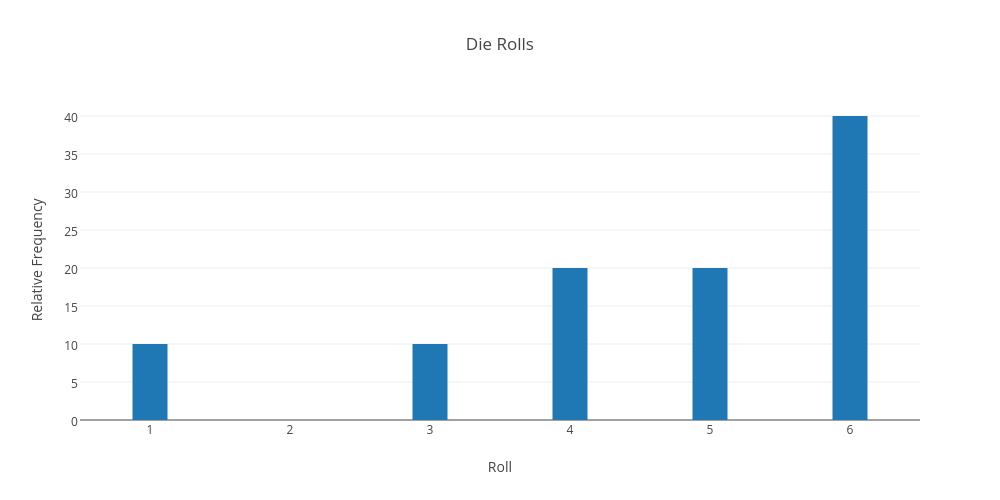
\includegraphics[scale = 0.3]{./images/die1.png}
\end{frame}

%%%%%%%%%%%%%%%%%%%%%%%%%%%%%%%%%%%%%%%%
\begin{frame}
\frametitle{100 Die Rolls}
	\centering
	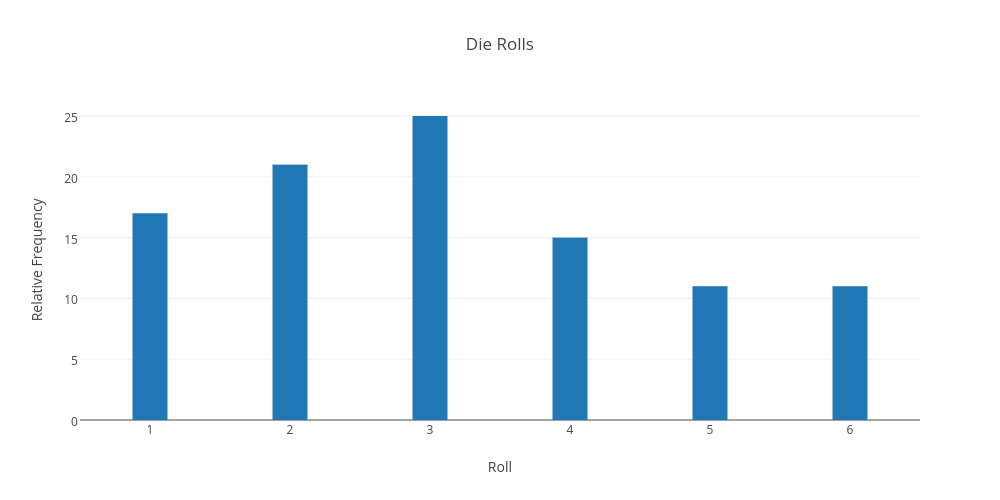
\includegraphics[scale = 0.3]{./images/die2.png}
\end{frame}

%%%%%%%%%%%%%%%%%%%%%%%%%%%%%%%%%%%%%%%%
\begin{frame}
\frametitle{1,000 Die Rolls}
	\centering
	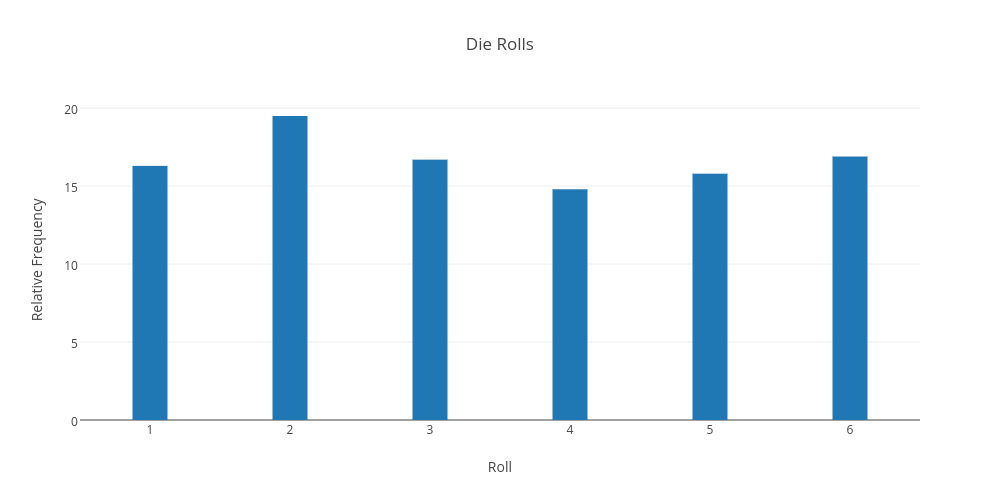
\includegraphics[scale = 0.3]{./images/die3.png}
\end{frame}

%%%%%%%%%%%%%%%%%%%%%%%%%%%%%%%%%%%%%%%%
\begin{frame}
\frametitle{1,000,000 Die Rolls}
	\centering
	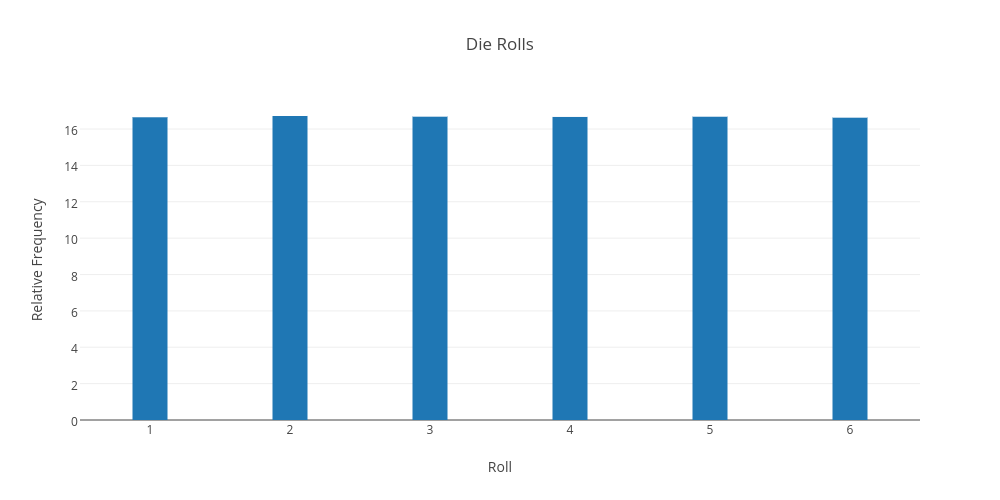
\includegraphics[scale = 0.3]{./images/die4.png}
\end{frame}

%%%%%%%%%%%%%%%%%%%%%%%%%%%%%%%%%%%%%%%%
\begin{frame}
\frametitle{What do you think of this argument?}
	\begin{itemize}
		\item The probability of flipping heads is 1/2: if we flip a coin many times, about half of the 
		time it will come up heads.
		\item The last ten throws in a row the coin has come up heads.
		\item The coin is bound to come up tails next time -- it would be very rare to get 11 heads in a 
		row.
	\end{itemize}
\end{frame}

%%%%%%%%%%%%%%%%%%%%%%%%%%%%%%%%%%%%%%%%
\begin{frame}
\frametitle{The Gambler's Fallacy}
	\alert{Relative frequencies settle down to probabilities, but this does not mean that the trials are 
	dependent.}
	
    \textbf{Dependent:} ``Memory'' of previous trials

	\textbf{Independent:} No ``memory'' of previous trials
\end{frame}

%%%%%%%%%%%%%%%%%%%%%%%%%%%%%%%%%%%%%%%%
\begin{frame}
\frametitle{Another Argument}
	\begin{quote}
	Lucie visits Albert. As she enters, he rolls four dice and shouts ``Hooray!'' for he has just rolled 
	four sixes. Lucie: ``I bet you've been rolling the dice for a long time to get that result!'' Now, Lucie 
	may have many reasons for saying this -- perhaps Albert is a lunatic dice-roller. But simply on the 
	evidence that he has just rolled four sixes, is her conclusion reasonable?
	\end{quote}
\end{frame}
%%%%%%%%%%%%%%%%%%%%%%%%%%%%%%%%%%%%%%%%
\begin{frame}
\frametitle{The \emph{Inverse} Gambler's Fallacy}
	\begin{block}{This is true:}
	    Albert is more likely to get four sixes if he rolls many times than if he rolls only once.
	\end{block}
	\begin{block}{However:} 
	    \emph{Regardless} of how long Albert has been rolling, the probability that he gets four sixes 
	    \alert{on the particular roll that Lucie observes} is unchanged. 
    \end{block}
	\vspace{2em}
	\textbf{The outcome of that roll doesn't tell us anything about whether he has rolled the dice 
	before, just like six heads in a row doesn't mean we're ``due'' for a tails.}
\end{frame}

%%%%%%%%%%%%%%%%%%%%%%%%%%%%%%%%%%%%%%%%
\begin{frame}
\frametitle{Definitions}
    \begin{itemize}
        \item \textbf{Random Experiment:} An experiment whose outcomes are random.
        \item \textbf{Basic Outcomes:} Possible outcomes (mutually exclusive) of random experiment.
        \item \textbf{Sample Space ($S$):} Set of all basic outcomes of a random experiment.
        \item \textbf{Event ($E$):} A subset of the \textit{sample space}. In set notation we write $E 
        \subseteq S$.
    \end{itemize}
\end{frame}

%%%%%%%%%%%%%%%%%%%%%%%%%%%%%%%%%%%%%%%%
\begin{frame}
\frametitle{Examples}
	\begin{itemize}
	    \item \textbf{Experiment:} Tossing a pair of dice.
	    \item \textbf{Basic Outcome:} An ordered pair $(a, b)$ where $a,b \in \{1, 2, 3, 4, 5, 6\}$, e.g.\ 
	    $(2,5)$
	    \item \textbf{Sample Space:} $S =$ \emph{All} ordered pairs $(a, b)$ where $a,b \in \{1, 2, 3, 4, 5, 
	    6\}$
        \item \textbf{Event:} $E$ = $\{(2,5), (5,5), (2,3), (3,2), (4,2), (5,3)\}$
    \end{itemize}
\end{frame}

%%%%%%%%%%%%%%%%%%%%%%%%%%%%%%%%%%%%%%%%
\begin{frame}
\frametitle{Visual Representation}
	\begin{figure}
	\centering
	\begin{tikzpicture}[scale = 1.4]
		\draw (0,0) circle [radius = 1];
		\draw (0,1)  node [text=black,above] {$E$};
	      \draw (-2,-2) rectangle (3,2);
	      \draw (3,2) node [text=black,above] {$S$};
	      \draw [fill] (2,0.5) circle [radius=0.03];
	      \draw (2,0.5) node [text=black,above] {$O_1$};
	      \draw [fill] (0.4,-0.5) circle [radius=0.03];
	      \draw (0.4,-0.5) node [text=black,above] {$O_2$};
	      \draw [fill] (-0.2,0.3) circle [radius=0.03];
	      \draw (-0.2,0.3) node [text=black,above] {$O_3$};
	\end{tikzpicture}
	\end{figure}
\end{frame}

%%%%%%%%%%%%%%%%%%%%%%%%%%%%%%%%%%%%%%%%
\begin{frame}
\frametitle{Our Example}
    \centering
    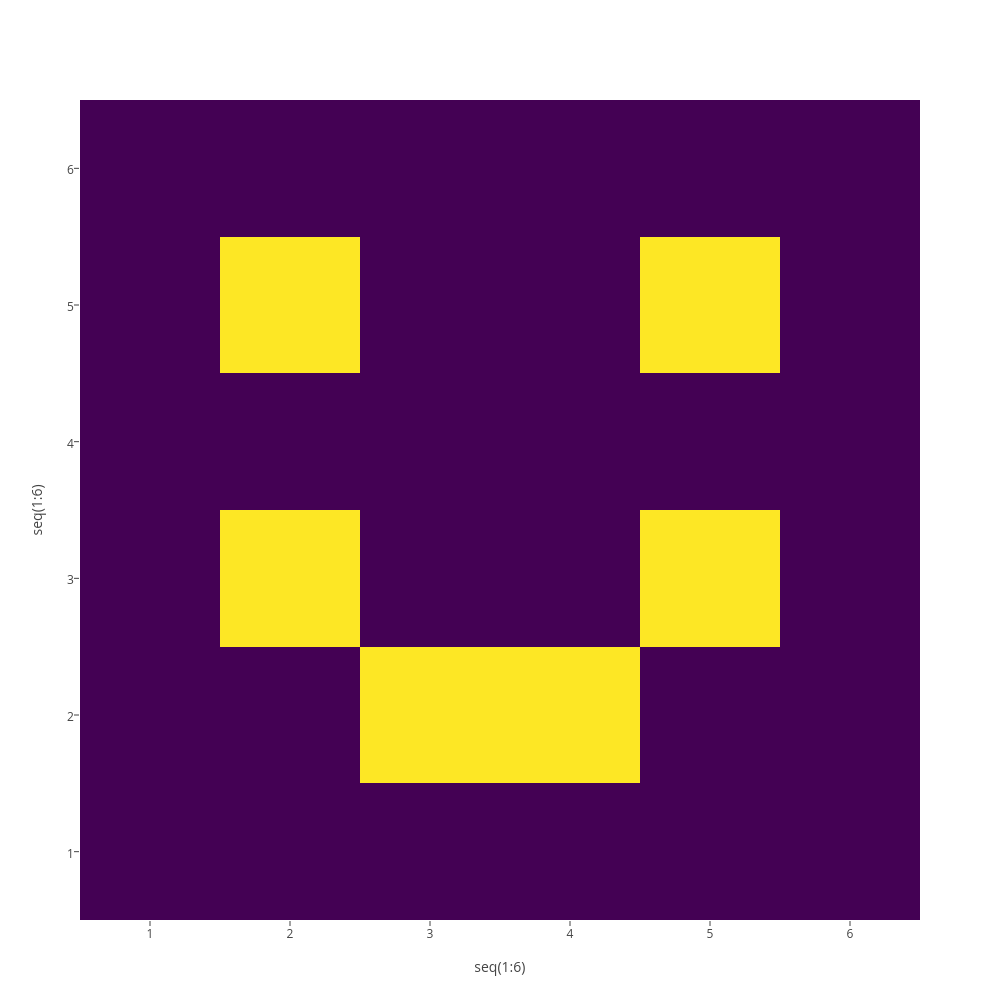
\includegraphics[scale=0.2]{./images/dieHeatMap.png}
\end{frame}

%%%%%%%%%%%%%%%%%%%%%%%%%%%%%%%%%%%%%%%%
\begin{frame}
	\begin{center}
		\Huge Probability is Defined on \emph{Sets}, and Events are Sets
	\end{center}
\end{frame}

%%%%%%%%%%%%%%%%%%%%%%%%%%%%%%%%%%%%%%%%
\begin{frame}
\frametitle{Dice Problem}
\end{frame}

\section{Set Theory}
%%%%%%%%%%%%%%%%%%%%%%%%%%%%%%%%%%%%%%%%
%Some macros for the Venn Diagrams
\def\eventA{(-0.35,0) circle (1.2)}
\def\eventB{(1.35,0) circle (1.2)}
\def\samplespace{(-2,-2) rectangle (3,2)}
%%%%%%%%%%%%%%%%%%%%%%%%%%%%%%%%%%%%%%%%
\begin{frame}
\frametitle{Complement of an Event: $A^c = \mbox{not } A$}
	\begin{figure}
	\centering
	\begin{tikzpicture}[scale = 1.2]	
		\fill[blue, fill opacity = 0.5] \samplespace;
		\fill[white, fill opacity = 1] \eventA;
	     	\draw \eventA node [above] {$A$};
	      \draw \samplespace (3,2) node [text=black,above] {$S$};	
	\end{tikzpicture}
	\caption{The complement $A^c$ of an event $A\subseteq S$ is the collection of all basic outcomes from $S$ not contained in $A$.}
	\end{figure}
\end{frame}

%%%%%%%%%%%%%%%%%%%%%%%%%%%%%%%%%%%%%%%%
\begin{frame}
\frametitle{Intersection of Events: $A\cap B = A \mbox{ and } B$}
	\begin{figure}
	\centering
	\begin{tikzpicture}[scale = 1.2]
	      \begin{scope}[fill opacity = 0.5]
	      \clip \eventA;
	      \fill[blue] \eventB;
	    \end{scope}
	     
	     	\draw \eventA node [above] {$A$};
		\draw \eventB node [above] {$B$};
	      \draw \samplespace (3,2) node [text=black,above] {$S$};
	      
	\end{tikzpicture}
	\caption{The intersection $A\cap B$ of two events $A,B\subseteq S$ is the collection of all basic 
	outcomes from $S$ contained in both $A$ and $B$}
	\end{figure}
\end{frame}

%%%%%%%%%%%%%%%%%%%%%%%%%%%%%%%%%%%%%%%%
\begin{frame}
\frametitle{Union of Events: $A\cup B = A \mbox{ or } B$}
	\begin{figure}
	\centering
	\begin{tikzpicture}[scale = 1.15]
	
		\begin{scope}[fill opacity = 0.5]
			\fill[blue] \eventA;
			\fill[red] \eventB;
		\end{scope}
		
		\draw \eventA node [above] {$A$};
		\draw \eventB node [above] {$B$};
	      \draw \samplespace node [text=black,above] {$S$};
	      
	\end{tikzpicture}
	\caption{The union $A\cup B$ of two events $A,B\subseteq S$ is the collection of all basic 
	outcomes from $S$ contained in $A$, $B$ or both.}
	\end{figure}
\end{frame}

%%%%%%%%%%%%%%%%%%%%%%%%%%%%%%%%%%%%%%%%
\begin{frame}
\frametitle{Quick Set Theory Result}
What is the formula for $A \cup B$?

\only<2->{
$$
A \cup B = A + B - (A \cap B)
$$
}
\end{frame}

%%%%%%%%%%%%%%%%%%%%%%%%%%%%%%%%%%%%%%%%
\begin{frame}
\frametitle{Mutually Exclusive and Collectively Exhaustive}
	\begin{block}{Mutually Exclusive Events}
		A collection of events $E_1, E_2, E_3, \hdots$ is \emph{\alert{mutually exclusive}} if $E_i \cap 
		E_j$ of \alert{\emph{any two different events}} is empty (formally $E_i \cap E_j = \emptyset$ 
		for any $i\neq j$).
	\end{block}
	
	\begin{block}{Collectively Exhaustive Events}
		A collection of events $E_1, E_2, E_3, \hdots$ is \emph{\alert{collectively exhaustive}} if, taken 
		together, they contain \alert{\emph{all of the basic outcomes in $S$}} (formally $E_1 \cup E_2 
		\cup \ldots  = S$).
	\end{block}
\end{frame}
%%%%%%%%%%%%%%%%%%%%%%%%%%%%%%%%%%%%%%%%
\begin{frame}
\frametitle{Implications}
	\begin{block}{Mutually Exclusive Events}
	      If one of the events occurs, then none of the others did.
	\end{block}
	
	\begin{block}{Collectively Exhaustive Events}
        One of these events \emph{must} occur.
	\end{block}
	
	Can you come up with examples of 
	\begin{itemize}
	    \item Mutually exclusive events that are not collectively exhaustive?
	    \item Collectively exhaustive events that are not mutually exclusive?
	\end{itemize}
\end{frame}

%%%%%%%%%%%%%%%%%%%%%%%%%%%%%%%%%%%%%%%%
%Some macros for collectively exhaustive and mutually exclusive sets
\def\Srect{(-2,-2) rectangle (4,2)}
\def\Arect{(-2,-2) rectangle (0,2)}
\def\Brect{(0,-2) rectangle (2,2)}
\def\Crect{(0,2) rectangle (4,2)}
\def\Devent{(1.6,-0.3) circle (1.3)}
\def\Eevent{(-1,1.2) circle (0.5)}
%%%%%%%%%%%%%%%%%%%%%%%%%%%%%%%%%%%%%%%%
\begin{frame}
\frametitle{Mutually Exclusive but \emph{not Collectively Exhaustive}}
\begin{figure}
\centering
\begin{tikzpicture}[scale = 1.2]
	\draw \Eevent node [above] {$A$};
	\draw \Devent node [above] {$B$};
      \draw \Srect node [above] {$S$};
\end{tikzpicture}
\caption{Although $A$ and $B$ don't overlap, they also don't cover $S$.}
%\caption{Although $A \cap B = \emptyset$, $A \cup B \neq S$}
\end{figure}
\end{frame}

%%%%%%%%%%%%%%%%%%%%%%%%%%%%%%%%%%%%%%%%
\begin{frame}
\frametitle{Collectively Exhaustive but \emph{not Mutually Exclusive}}
\begin{figure}
\centering
\begin{tikzpicture}[scale = 1.2]

	\draw \Arect node [below left] {$A$};
	\draw \Brect node [below left] {$B$};
	\draw \Crect node [below left] {$C$};
	\draw \Devent node [above] {$D$};
      \draw \Srect node [above] {$S$};
\end{tikzpicture}
\caption{Together $A, B, C$ and $D$ cover $S$, but $D$ overlaps with $B$ and $C$.}
\end{figure}
\end{frame}

%%%%%%%%%%%%%%%%%%%%%%%%%%%%%%%%%%%%%%%%
\begin{frame}
\frametitle{Collectively Exhaustive \emph{and} Mutually Exclusive}
\begin{figure}
\centering
\begin{tikzpicture}[scale = 1.2]

	\draw \Arect node [below left] {$A$};
	\draw \Brect node [below left] {$B$};
	\draw \Crect node [below left] {$C$};
      \draw \Srect node [above] {$S$};
\end{tikzpicture}
\caption{$A$, $B$, and $C$ cover $S$ and don't overlap.}
\end{figure}
\end{frame}

%%%%%%%%%%%%%%%%%%%%%%%%%%%%%%%%%%%%%%%%
%Some macros for the Venn Diagrams
\def\EventA{(-0.35,0) circle (1.2)}
\def\EventB{(1.35,0) circle (1.2)}
\def\EventC{(-0.35,0) circle (0.6)}
\def\EventD{(0,0) circle (1.6)}
\def\SampleSpace{(-2,-2) rectangle (3,2)}
%%%%%%%%%%%%%%%%%%%%%%%%%%%%%%%%%%%%%%%%
\begin{frame}
	\frametitle{The Complement Rule: $P(A^c) = 1- P(A)$}
	\begin{columns}
	
\column{0.7\textwidth}
\uncover<1->{Since $A, A^c$ are \textit{mutually exclusive} and \textit{collectively exhaustive}:}
$$\uncover<2->{P(A \cup A^c) =} \uncover<2->{P(A) + P(A^c) =} \uncover<3->{P(S) =} \uncover<3->{1}$$
\uncover<4->{Rearranging:}
	\uncover<4->{$$P(A^c) = 1 - P(A)$$}
\column{0.3\textwidth}
\uncover<1->{
\begin{figure}
\centering
\begin{tikzpicture}[scale = 0.6]
	\draw (1.8,0.8) node [above]{$A^c$};
	\draw \EventA node [above] {$A$};
      \draw \SampleSpace node [text=black,above] {$S$};
\end{tikzpicture}
\caption{$A\cap A^c = \emptyset$, $A \cup A^c = S$}
\end{figure}}

\end{columns}
\end{frame}

%%%%%%%%%%%%%%%%%%%%%%%%%%%%%%%%%%%%%%%%
\begin{frame}
\frametitle{Will Having 5 Children Guarantee a Boy? }
A couple plans to have five children. Assuming that each birth is independent and male and female children are equally likely, what is the probability that they have at least one boy?
\vspace{1em}

\pause
\alert{By Independence and the Complement Rule,}
	\begin{align*}
		P(\mbox{no boys})&= P(\mbox{5 girls})\\
							&= 1/2 \times 1/2 \times 1/2 \times 1/2 \times 1/2\\
							&=\ 1/32\\
		P(\mbox{at least 1 boy})&=1 - P(\mbox{no boys})\\
		&=1 - 1/32 =31/32 = 0.97
	\end{align*}

\end{frame}

%%%%%%%%%%%%%%%%%%%%%%%%%%%%%%%%%%%%%%%%
\begin{frame}
\frametitle{The Birthday Problem}
	\begin{quote}
		What is the least number of persons required if the probability exceeds 1/2 that two or more of them have the same birthday? (Year of birth need not match.)
	\end{quote}
	
	\hfill \alert{[Hint: Use the Complement Rule.]}
\end{frame}

%%%%%%%%%%%%%%%%%%%%%%%%%%%%%%%%%%%%%%%%
\begin{frame}
\frametitle{Coin Flipping}
\end{frame}

%%%%%%%%%%%%%%%%%%%%%%%%%%%%%%%%%%%%%%%%

\begin{frame}
\frametitle{Axioms of Probability}
We assign every event $A$ in the sample space $S$ a real number $P(A)$ called the \alert{probability of $A$} such that: 
\vspace{1em}
\begin{description}
	\item[Axiom 1] $0 \leq P(A) \leq 1$
	\item[Axiom 2] $P(S)=1$
	\item[Axiom 3] If $A_1, A_2, A_3, \hdots$ are mutually exclusive events, then $P(A_1\cup A_2 \cup A_3 \cup \cdots) = P(A_1) + P(A_2) + P(A_3) + \hdots$
\end{description}

\end{frame}

%%%%%%%%%%%%%%%%%%%%%%%%%%%%%%%%%%%%%%%%
\begin{frame}
\frametitle{Equivalent Events}

\begin{block}{If A and B are Logically Equivalent, then $P(A) = P(B)$.}\end{block}

\begin{alertblock}{In other words, if A and B contain exactly the same basic outcomes, then $P(A) = P(B)$.}\end{alertblock}

Although this seems obvious it's important to keep in mind, especially later in the course...
\end{frame}
%%%%%%%%%%%%%%%%%%%%%%%%%%%%%%%%%%%%%%%%
\begin{frame}
\frametitle{The Logical Consequence Rule}

\begin{block}{If B Logically Entails A, then $P(B)\leq P(A)$}\end{block}

\begin{alertblock}{In other words, $B\subseteq A \Rightarrow P(B)\leq P(A)$}\end{alertblock}


\begin{block}{Why is this so?}
If $B \subseteq A$, then all the basic outcomes in $B$ are also in $A$.
\end{block}

\end{frame}
%%%%%%%%%%%%%%%%%%%%%%%%%%%%%%%%%%%%%%%%

\begin{frame}
\frametitle{Proof of Logical Consequence Rule}
	\begin{columns}
	
\column{0.75\textwidth}
\uncover<1->{Since $B \subseteq A$, we have $B = A\cap B$ and $A = B \cup (A \cap B^c)$.}\uncover<1->{ Combining these,
	$$A = (A \cap B) \cup (A \cap B^c)$$}
\uncover<1->{Now since $(A \cap B) \cap (A \cap B^c) = \emptyset$,}
\begin{eqnarray*}
	\uncover<1->{P(A) &=& P(A \cap B)  + P(A \cap B^c)\\}
	\uncover<1->{&=&  P(B) + P(A \cap B^c)\\}
	\uncover<1->{&\geq& P(B)}
\end{eqnarray*}
\uncover<1->{because $0 \leq P(A \cap B^c) \leq 1$.}
\column{0.25\textwidth}
\uncover<1->{\begin{figure}
\centering
\begin{tikzpicture}[scale = 0.48]
	\draw \EventC;
	\draw \EventD;
	\draw (0, 0.5) node [above] {$A$};
	\draw (-0.3, -0.5) node [above] {$B$};
      \draw \SampleSpace node [text=black,above] {$S$};
\end{tikzpicture}
\caption{$B = A\cap B$, and $A = B \cup (A \cap B^c)$}
\end{figure}}

\end{columns}


\end{frame}

\section{Permutations and Combinations}
%%%%%%%%%%%%%%%%%%%%%%%%%%%%%%%%%%%%%%%%

\begin{frame}

\frametitle{``Classical'' Probability}

When all of the basic outcomes are equally likely, the probability of an event is simply the total number of basic outcomes that make up the event divided by the total number of basic outcomes.

\end{frame}
%%%%%%%%%%%%%%%%%%%%%%%%%%%%%%%%%%%%%%%%
\begin{frame}
\frametitle{Recall from High School Math:}

\begin{block}{Multiplication Rule for Counting}
$n_1$ ways to make first decision, $n_2$ ways to make second, $\hdots, n_k$ ways to make kth $\Rightarrow n_1 \times n_2 \times \cdots \times n_k$ total ways to decide. \end{block}
\begin{block}{Corollary -- Number of Possible Orderings}
$k \times(k-1)\times (k-2) \times \cdots\times  2 \times 1 = k!$
\end{block}

\begin{block}{Permutations -- Order $n$ people in $k$ slots}
$P_k^n = \frac{n!}{(n-k)!}$\end{block}

\begin{block}{Combinations -- Choose committee of $k$ from group of $n$}
$\binom{n}{k} = \frac{n!}{k! \, (n-k)!}$, where $0! = 1$\end{block}

\end{frame}

%%%%%%%%%%%%%%%%%%%%%%%%%%%%%%%%%%%%%%%%
\begin{frame}
\frametitle{Cards, Tennis, and Obama}
\end{frame}

\section{Conditional Probability}
%%%%%%%%%%%%%%%%%%%%%%%%%%%%%%%%%%%%%%%%
\begin{frame}
\frametitle{Conditional Probability -- Reduced Sample Space}
$$
P(A|B) = \frac{P(A\cap B)}{P(B)},\;\; P(B)>0
$$
\begin{figure}
\centering
\begin{tikzpicture}[scale = 0.77]

	\begin{scope}[fill opacity = 0.5]
		\fill[red] \EventB;
      	\clip \EventA;
      	\fill[blue] \EventB;
    \end{scope}
	\draw \EventA node [above] {$A$};
	\draw \EventB node [above] {$B$};
      \draw \SampleSpace node [right] {$S$};
\end{tikzpicture}
\caption{$B$ becomes the ``new sample space'' so we need to re-scale by $P(B)$ to keep probabilities between zero and one.}
\end{figure}
\end{frame}
%%%%%%%%%%%%%%%%%%%%%%%%%%%%%%%%%%%%%%%%
\begin{frame}
\frametitle{Who's on the other side?}
Let $F$ be the event that Obama is on the front of the card of the card we draw and $B$ be the event that he is on the back.
$$P(B|F) = \frac{P(B\cap F)}{P(F)} = \pause \alert{\frac{1/3}{1/2}= \pause 2/3}$$

\end{frame}

%%%%%%%%%%%%%%%%%%%%%%%%%%%%%%%%%%%%%%%%
\begin{frame}
  \small
  \begin{block}{Conditional Versions of Probability Axioms}
    \begin{enumerate}
      \item $0 \leq P(A|B) \leq 1$
      \item $P(B|B) = 1$
      \item If $A_1, A_2, A_3, \dots$ are mutually exclusive events, then $P(A_1\cup A_2\cup A_3 \cup \cdots|B) = P(A_1|B) + P(A_2|B) + P(A_3|B)\dots$
    \end{enumerate}
  \end{block}

  \begin{block}{Conditional Versions of Other Probability Rules}
    \begin{itemize}
      \item $P(A|B) = 1 - P(A^c|B)$
      \item $A_1$ logically equivalent to $A_2 \iff P(A_1|B) = P(A_2|B)$
      \item $A_1 \subseteq A_2 \implies P(A_1|B) \leq P(A_2|B)$  
      \item $P(A_1 \cup A_2 | B) = P(A_1|B) + P(A_2|B) - P(A_1 \cap A_2|B)$
    \end{itemize}
  \end{block}

    \alert{However: $P(A|B) \neq P(B|A)$ and $P(A|B^c) \neq 1 - P(A|B)$!}
  
\end{frame}
%%%%%%%%%%%%%%%%%%%%%%%%%%%%%%%%%%%%%%%%
\begin{frame}
\frametitle{Independence and The Multiplication Rule}
\begin{block}{The Multiplication Rule}
Rearrange the definition of conditional probability:
$P(A\cap B) = P(A|B)P(B)$
\end{block}\pause
\begin{block}{Statistical Independence}
$P(A\cap B) = P(A)P(B)$
\end{block}\pause
\begin{alertblock}{By the Multiplication Rule}
$\mbox{Independence } \iff P(A|B) = P(A)$\\
\end{alertblock}\pause
\begin{block}{Interpreting Independence}
Knowing $B$ has occurred tells nothing about whether $A$ will.
\end{block}
\end{frame}

\section{The Law of Total Probability}
%%%%%%%%%%%%%%%%%%%%%%%%%%%%%%%%%%%%%%%%
\begin{frame}
\frametitle{The Law of Total Probability}
If $E_1, E_2, \hdots, E_k$ are mutually exclusive, collectively exhaustive events and $A$ is another event, then
	$$P(A) = P(A|E_1)P(E_1) + P(A|E_2)P(E_2) + \hdots + P(A|E_k)P(E_k)$$

\end{frame}

%%%%%%%%%%%%%%%%%%%%%%%%%%%%%%%%%%%%%%%%
\begin{frame}
  \frametitle{Example of Law of Total Probability}
  Define the following events:
  \begin{align*}
    F &=  \mbox{Obama on front of card}\\
    A &=  \mbox{Draw card with two Gagas}\\
    B &=  \mbox{Draw card with two Obamas}\\
    C &=  \mbox{Draw card with BOTH Obama and Gaga}\\
    \\
  P(F) &= P(F|A)P(A) + P(F|B)P(B) + P(F|C)P(C) \\
 \only<2->{ &= 0 \times 1/3 + 1 \times 1/3 + 1/2 \times 1/3 \\
  &= 1/2}
  \end{align*}

\end{frame}
%%%%%%%%%%%%%%%%%%%%%%%%%%%%%%%%%%%%%%%%
%Some macros for the Venn Diagrams
\def\EventA{(-0.35,0) circle (1.2)}
\def\EventB{(1.35,0) circle (1.2)}
\def\EventC{(-0.35,0) circle (0.6)}
\def\EventD{(0,0) circle (1.6)}
\def\SampleSpace{(-2,-2) rectangle (3,2)}
%%%%%%%%%%%%%%%%%%%%%%%%%%%%%%%%%%%%%%%%
\begin{frame}
\frametitle{Deriving the Law of Total Probability For $k=2$}

\begin{columns}

\column{0.7\textwidth}
\uncover<2->{

Since $A\cap B$ and $A \cap B^c$ are mutually exclusive and their union equals $A$,
	$$P(A) = P(A\cap B) + P(A \cap B^c)$$}
	\uncover<3->{
But by the multiplication rule:
	\begin{align*}
		P(A\cap B)&=P(A|B)P(B)\\
		P(A \cap B^c)&=P(A|B^c)P(B^c)
	\end{align*}}
\uncover<4->{
Combining,
	$$\alert{P(A) = P(A|B)P(B) + P(A|B^c)P(B^c)}$$}
\column{0.3\textwidth}
\uncover<1->{
\begin{figure}
\centering
\begin{tikzpicture}[scale = 0.5]

	\begin{scope}[fill opacity = 0.5]
		\fill[red] \EventB;
      	\clip \EventA;
      	\fill[blue] \EventB;
    \end{scope}
	\draw \EventA node [above] {$B$};
	\draw \EventB node [above] {$A$};
      \draw \SampleSpace node [right] {$S$};
\end{tikzpicture}
\caption{$A = (A\cap B) \cup (A \cap B^c)$, $(A\cap B) \cap (A \cap B^c) = \emptyset$}
\end{figure}}

\end{columns}

\end{frame}

\section{Prediction Markets}
%%%%%%%%%%%%%%%%%%%%%%%%%%%%%%%%%%%%%%%%

\begin{frame}

\frametitle{How do prediction markets work?}
\begin{center}
\fbox{\fbox{\begin{minipage}{0.8\textwidth}
  \textsc{This certificate entitles the bearer to \$1 if Trump wins the 2016 US presidential election.}
\end{minipage}}}
\vspace{1em}

\begin{block}{Buyers -- Purchase Right to Collect}
Trump very likely to win $\Rightarrow$ buy for close to \$1. \\Trump very unlikely to win $\Rightarrow$ buy for close to \$0.
\end{block}

\begin{block}{Sellers -- Sell Obligation to Pay} 
Trump very likely to win $\Rightarrow$ sell for close to \$1. \\Trump very unlikely to win $\Rightarrow$ sell for close to \$0.
\end{block}
\end{center}

\end{frame}
%%%%%%%%%%%%%%%%%%%%%%%%%%%%%%%%%%%%%%%%
\begin{frame}
\frametitle{Probabilities from Prediction Markets}

  \begin{block}{Probabilities from Beliefs}
    Market price of contract encodes market participants' beliefs in the form of probability:
$$\mbox{Price}/\mbox{Payout}\approx \mbox{Subjective Probability}$$
  \end{block} \pause

	\begin{alertblock}{Statistical Arbitrage}
    If the probabilities implied by prediction market prices violate \emph{any} of our probability rules there is a \emph{pure arbitrage opportunity}: a way make to make a guaranteed, risk-free profit.
	\end{alertblock}

\end{frame}
%%%%%%%%%%%%%%%%%%%%%%%%%%%%%%%%%%%%%%%%
\begin{frame}
\frametitle{A Simple Example of Statistical Arbitrage}

\begin{block}{November 5th, 2012}
	\begin{itemize}
		\item\$2.30 for contract paying \$10 if Romney wins on BetFair
		\item \$6.58 for contract paying \$10 if Obama wins on InTrade
	\end{itemize}
\end{block}

\begin{block}{Implied Probabilities}
	\begin{itemize}
	\item BetFair: $P(Romney) \approx 0.23$
	\item InTrade: $P(Obama) \approx 0.66$
	\end{itemize}
\end{block}

\begin{alertblock}{What's Wrong with This?}\pause
 Violates complement rule! $P(Obama) = 1 - P(Romney)$ but the implied probabilities here don't sum up to one!
\end{alertblock}



\end{frame}

%%%%%%%%%%%%%%%%%%%%%%%%%%%%%%%%%%%%%%%%
\begin{frame}
\frametitle{A Simple Example of Statistical Arbitrage}
\framesubtitle{Courtesy of  \fbox{\href{http://offsettingbehaviour.blogspot.co.nz/2012/11/barriers-to-arbitrage.html}{Eric Crampton}}}

\begin{block}{November 5th, 2012}
	\begin{itemize}
		\item\$2.30 for contract paying \$10 if Romney wins on BetFair
		\item \$6.58 for contract paying \$10 if Obama wins on InTrade
	\end{itemize}
\end{block}

\begin{alertblock}{Arbitrage Strategy}
Buy Equal Numbers of Each 
	\begin{itemize}
		\item Cost = \$2.30 + \$6.58 =\$8.88 per pair 
		\item Payout if Romney Wins: \$10 
		\item Payout if Obama Wins: \$10
		\item Guaranteed Profit: \$10 - \$8.88 = \$1.12 per pair
	\end{itemize} 

\end{alertblock}

\end{frame}

\section{The Lie Detector}
%%%%%%%%%%%%%%%%%%%%%%%%%%%%%%%%%%%%%%%%
\begin{frame}
\frametitle{The Lie Detector Problem}
\begin{block}{From accounting records, we know that 10\% of employees in the store are stealing merchandise.}
\end{block}
\begin{block}{The managers want to fire the thieves, but their only tool in distinguishing is a lie detector test that is 80\% accurate:}
	\begin{eqnarray*}
	\mbox{Innocent } &\Rightarrow& \mbox{Pass test with } 80\% \mbox{ Probability}\\
	\mbox{Thief} &\Rightarrow& \mbox{Fail test with } 80\% \mbox{ Probability}
	\end{eqnarray*}
\end{block}

\pause
\begin{alertblock}{What is the probability that someone is a thief \emph{given} that she has failed the lie detector test? }
\end{alertblock}

\end{frame}
%%%%%%%%%%%%%%%%%%%%%%%%%%%%%%%%%%%%%%%%

\begin{frame}
\frametitle{Monte Carlo Simulation}
Managers will split up and visit employees. Employees roll the die twice \alert{but keep the results secret!}
\vspace{1em}
\begin{block}{First Roll -- Thief or not?}
$0 \Rightarrow$ Thief, $1-9 \Rightarrow$ Innocent
\end{block}

\begin{block}{Second Roll -- Lie Detector Test}
$0,1 \Rightarrow$ Incorrect Test Result, $2-9$ Correct Test Result
\end{block}
\begin{table}
	\begin{tabular}{l|cc}
	&0 or 1&2--9\\
	\hline
	Thief (0)&Pass&\alert{Fail}\\
	Innocent ($>0$)&\alert{Fail} &Pass
	\end{tabular}
\end{table}

\end{frame}
%%%%%%%%%%%%%%%%%%%%%%%%%%%%%%%%%%%%%%%%
\begin{frame}
\frametitle{What percentage of those who failed the test are guilty?}
\begin{block}{\# Who Failed Lie Detector Test:}

\end{block}


\begin{block}{\# Of Thieves Among Those Who Failed:}

\end{block}

\end{frame}
%%%%%%%%%%%%%%%%%%%%%%%%%%%%%%%%%%%%%%%%
\begin{frame}
\frametitle{Base Rate Fallacy -- Failure to Consider Prior Information}

\begin{block}{Base Rate -- Prior Information}
Before the test we know that 10\% of Employees are stealing.
\end{block}
\vspace{2em}
\begin{alertblock}{People tend to focus on the fact that the test is 80\% accurate and ignore the fact that only 10\% of the employees are theives. }
\end{alertblock}

\end{frame}
%%%%%%%%%%%%%%%%%%%%%%%%%%%%%%%%%%%%%%%%
\begin{frame}
\frametitle{Thief (Y/N), Lie Detector (P/F)}
\footnotesize
\begin{table}
\begin{tabular}{|c|cccccccccc|}
\hline
&0&1&2&3&4&5&6&7&8&9\\
\hline
0&\textcolor{blue}{YP}&\textcolor{blue}{YP}&\textcolor{red}{YF}&\textcolor{red}{YF}&\textcolor{red}{YF}&\textcolor{red}{YF}&\textcolor{red}{YF}&\textcolor{red}{YF}&\textcolor{red}{YF}&\textcolor{red}{YF}\\
1&\textcolor{red}{NF}&\textcolor{red}{NF}&\textcolor{blue}{NP}&\textcolor{blue}{NP}&\textcolor{blue}{NP}&\textcolor{blue}{NP}&\textcolor{blue}{NP}&\textcolor{blue}{NP}&\textcolor{blue}{NP}&\textcolor{blue}{NP}\\
2&\textcolor{red}{NF}&\textcolor{red}{NF}&\textcolor{blue}{NP}&\textcolor{blue}{NP}&\textcolor{blue}{NP}&\textcolor{blue}{NP}&\textcolor{blue}{NP}&\textcolor{blue}{NP}&\textcolor{blue}{NP}&\textcolor{blue}{NP}\\
3&\textcolor{red}{NF}&\textcolor{red}{NF}&\textcolor{blue}{NP}&\textcolor{blue}{NP}&\textcolor{blue}{NP}&\textcolor{blue}{NP}&\textcolor{blue}{NP}&\textcolor{blue}{NP}&\textcolor{blue}{NP}&\textcolor{blue}{NP}\\
4&\textcolor{red}{NF}&\textcolor{red}{NF}&\textcolor{blue}{NP}&\textcolor{blue}{NP}&\textcolor{blue}{NP}&\textcolor{blue}{NP}&\textcolor{blue}{NP}&\textcolor{blue}{NP}&\textcolor{blue}{NP}&\textcolor{blue}{NP}\\
5&\textcolor{red}{NF}&\textcolor{red}{NF}&\textcolor{blue}{NP}&\textcolor{blue}{NP}&\textcolor{blue}{NP}&\textcolor{blue}{NP}&\textcolor{blue}{NP}&\textcolor{blue}{NP}&\textcolor{blue}{NP}&\textcolor{blue}{NP}\\
6&\textcolor{red}{NF}&\textcolor{red}{NF}&\textcolor{blue}{NP}&\textcolor{blue}{NP}&\textcolor{blue}{NP}&\textcolor{blue}{NP}&\textcolor{blue}{NP}&\textcolor{blue}{NP}&\textcolor{blue}{NP}&\textcolor{blue}{NP}\\
7&\textcolor{red}{NF}&\textcolor{red}{NF}&\textcolor{blue}{NP}&\textcolor{blue}{NP}&\textcolor{blue}{NP}&\textcolor{blue}{NP}&\textcolor{blue}{NP}&\textcolor{blue}{NP}&\textcolor{blue}{NP}&\textcolor{blue}{NP}\\
8&\textcolor{red}{NF}&\textcolor{red}{NF}&\textcolor{blue}{NP}&\textcolor{blue}{NP}&\textcolor{blue}{NP}&\textcolor{blue}{NP}&\textcolor{blue}{NP}&\textcolor{blue}{NP}&\textcolor{blue}{NP}&\textcolor{blue}{NP}\\
9&\textcolor{red}{NF}&\textcolor{red}{NF}&\textcolor{blue}{NP}&\textcolor{blue}{NP}&\textcolor{blue}{NP}&\textcolor{blue}{NP}&\textcolor{blue}{NP}&\textcolor{blue}{NP}&\textcolor{blue}{NP}&\textcolor{blue}{NP}\\
\hline
\end{tabular}
\caption{Each outcome in the table is equally likely. The 26 given in red correspond to failing the test, but only 8 of these (YF) correspond to being a thief.}
\end{table}
\end{frame}
%%%%%%%%%%%%%%%%%%%%%%%%%%%%%%%%%%%%%%%%
\begin{frame}
\frametitle{Base Rate of Thievery is 10\%}

% Set the overall layout of the tree
\tikzstyle{level 1}=[level distance=3.5cm, sibling distance=3.5cm]
\tikzstyle{level 2}=[level distance=3.5cm, sibling distance=2.5cm]

% Define styles for bags and leafs
\tikzstyle{bag} = [text width=4em, text centered]
\tikzstyle{end} = [circle, minimum width=3pt,fill, inner sep=0pt]
\tikzstyle{tip} = [circle,fill, minimum height = 3pt, inner sep=0pt]
\begin{figure}
\centering
\begin{tikzpicture}[scale = 0.7,thick,grow=right]
\node[tip]{}
    child {
        node[bag] {Thief}        
        child {
                node[end, label=right:
                    {\alert{\fbox{Fail} $\;\;\; \frac{1}{10} \times \frac{4}{5} = \frac{4}{50}$}}] {}
                edge from parent
                node[below]  {$\frac{4}{5}$}
            }
            child {
                node[end, label=right:
                    {Pass}] {}
                edge from parent
                node[above] {$\frac{1}{5}$}
            }
            edge from parent 
            node[below]  {$\frac{1}{10}$}
    }
    child {
        node[bag] {Honest}        
        child {
                node[end, label=right:
                    {\alert{\fbox{Fail} $\;\;\; \frac{9}{10} \times \frac{1}{5} = \frac{9}{50}$}}] {}
                edge from parent
                node[below]  {$\frac{1}{5}$}
            }
            child {
                node[end, label=right:
                    {Pass}] {}
                edge from parent
                node[above] {$\frac{4}{5}$}
            }
        edge from parent         
            node[above] {$\frac{9}{10}$}
    };
\end{tikzpicture}
\caption{Although $\frac{9}{50} + \frac{4}{50} = \frac{13}{50}$ fail the test, only $\frac{4/50}{13/50} = \frac{4}{13} \approx 0.31$ are actually theives!}
\end{figure}


\end{frame}

\section{Bayes' Rule}
%%%%%%%%%%%%%%%%%%%%%%%%%%%%%%%%%%%%%%%%
\begin{frame}
\frametitle{Deriving Bayes' Rule}
Intersection is symmetric: $A\cap B = B\cap A$ so $P(A\cap B) = P(B \cap A)$ \pause  By the definition of conditional probability,
	$$P(A|B) = \frac{P(A\cap B)}{P(B)}$$ \pause
And by the multiplication rule:
	$$P(B\cap A) = P(B|A)P(A)$$ \pause
Finally, combining these
	$$P(A|B) = \frac{P(B|A)P(A)}{P(B)}$$
\end{frame}
%%%%%%%%%%%%%%%%%%%%%%%%%%%%%%%%%%%%%%%%
\begin{frame}
\frametitle{Understanding Bayes' Rule}
$$\boxed{P(A|B) = \frac{P(B|A)P(A)}{P(B)}}$$

\begin{block}
	{Reversing the Conditioning}
	Express $P(A|B)$ in terms of $P(B|A)$. \emph{Relative magnitudes} of the two conditional probabilities determined by the ratio $P(A)/P(B)$.
\end{block}

\begin{block}
	{Base Rate}
	$P(A)$ is called the ``base rate'' or the ``prior probability.'' 
\end{block}

\begin{block}
	{Denominator}
	Typically, we calculate $P(B)$ using the law of total probability
\end{block}


\end{frame}

%%%%%%%%%%%%%%%%%%%%%%%%%%%%%%%%%%%%%%%%
\begin{frame}
\frametitle{Solving the Lie Detector Problem with Bayes' Rule}
\footnotesize
\fbox{$T =$ Employee is a Thief, $F = $ Employee Fails Lie Detector Test}
\normalsize
$$P(T|F) = \frac{P(F|T)P(T)}{P(F)}$$ \pause
\begin{align*}
	P(F) &= P(F|T)P(T) + P(F|T^c)P(T^c)\\
		&= 0.8 \times 0.1 + 0.2\times 0.9\\ 
		&= \alert{0.08} + 0.18 = \alert{0.26} 
\end{align*}


$$P(T|F) = \frac{\alert{0.08}}{\alert{0.26}} = \pause \frac{8}{26} = \frac{4}{13} \approx 0.31$$
\end{frame}
%%%%%%%%%%%%%%%%%%%%%%%%%%%%%%%%%%%%%%%%
\begin{frame}
\singlespacing
\frametitle{``Odd'' Question \# 5}


There are two kinds of taxis: green cabs and blue cabs. Of all the cabs on the road, \alert{85\% are green cabs}. On a misty winter night a taxi sideswiped another car and drove off. \alert{A witness says it was a blue cab.} The witness is tested under conditions like those on the night of the accident, and \alert{80\% of the time she correctly reports the color of the cab that is seen}. That is, regardless of whether she is shown a blue or a green cab in misty evening light, she gets the color right 80\% of the time. 

\vspace{1em}
\begin{center}
\fbox{\begin{minipage}{0.85\textwidth}
\textcolor{blue}{Given that the witness said she saw a blue cab, what is the probability that a blue cab was the sideswiper?}
\end{minipage}}
\end{center}

\end{frame}

%%%%%%%%%%%%%%%%%%%%%%%%%%%%%%%%%%%%%%%%
\begin{frame}
\frametitle{Solving The Taxi Problem}
\footnotesize
\fbox{
\begin{minipage}{0.85\textwidth}
$G = $ Taxi is Green, $P(G) = 0.85$\\
$B = $ Taxi is Blue, $P(B) = 0.15$\\
$W_B = $ Witness says Taxi is Blue, $P(W_B|B) = 0.8, P(W_B|G) = 0.2$
\end{minipage}}
\normalsize

\pause
$$P(B|W_B) = P(W_B|B)P(B)/P(W_B)$$
\pause
\begin{align*}
	P(W_B) &= P(W_B|B) P(B) + P(W_B|G) P(G)\\ \pause
			&= 0.8\times 0.15 + 0.2 \times 0.85 \\ \pause
			&= \alert{0.12} + 0.17 = \alert{0.29}\\ \\ \pause
		P(B|W_B) &= 0.12/0.29 = 12/29 \approx 0.41\\ \pause
		P(G|W_B) &= 1 - (12/19) \approx 0.59 
	\end{align*}

\end{frame}

%%%%%%%%%%%%%%%%%%%%%%%%%%%%%%%%%%%%%%%%
\begin{frame}
\frametitle{The Monty Hall Problem!}
\begin{figure}
\includegraphics[scale = 0.28]{./images/door}
\includegraphics[scale = 0.28]{./images/door}
\includegraphics[scale = 0.28]{./images/door}
\end{figure}
\begin{figure}
	\fbox{\includegraphics[scale = 0.08]{./images/car}}
	\hspace{0.5em}
	\fbox{\includegraphics[scale = 0.095]{./images/goat}}
	\hspace{0.5em}
	\fbox{\includegraphics[scale = 0.095]{./images/goat}}
\end{figure}
\end{frame}
%%%%%%%%%%%%%%%%%%%%%%%%%%%%%%%%%%%%%%%%


\begin{frame}
\frametitle{What is the probability that you win if you switch? }
\begin{figure}
\centering
	\includegraphics[scale = 0.55]{./images/monty_hall}
\end{figure}
\end{frame}

%%%%%%%%%%%%%%%%%%%%%%%%%%%%%%%%%%%%%%%%%
\begin{frame}

\Huge Key Point -- Monte doesn't choose a door randomly: he \emph{always} shows you a goat.

\end{frame}
%%%%%%%%%%%%%%%%%%%%%%%%%%%%%%%%%%%%%%%%


\begin{frame}
\frametitle{Without loss of generality, suppose you chose door \#1}
\begin{figure}[htbp]
\begin{center}
\small
\synttree[Choose Door 1
			[\emph{Car Behind Door 1}
				[Switch	[\textbf{Lose}]	]	[Don't Switch	[\textbf{Win}]	]
			]
						[\emph{Car Behind Door 2}
				[Switch	[\textbf{Win}]	]	[Don't Switch	[\textbf{Lose}]	]
			]
						[\emph{Car Behind Door 3}
				[Switch	[\textbf{Win}]	]	[Don't Switch	[\textbf{Lose}]	]
			]
]
\end{center}
\end{figure}
\end{frame}

%%%%%%%%%%%%%%%%%%%%%%%%%%%%%%%%%%%%%%%
\end{document}
